% ============================================================================
%  Section: End-to-end Timing Distribution
%
%  Updated to reflect the persistent backend worker architecture (n=30, 4-inst
%  cross-region deployment). Previous spawn-per-request data is retained in
%  the comparison below (Spawn baseline) but the headline numbers now report
%  the production-default worker mode.
%
%  Required packages (add to preamble if not already present):
%    \usepackage{graphicx}
%    \usepackage{booktabs}
%
%  Required figure files (place in figures/):
%    figures/fig_wall_total_cdf.pdf  (or .png)
% ============================================================================

\subsubsection{End-to-end Timing Distribution}
\label{sec:e2e-timing}

% ----------------------------------------------------------------------------
% Experimental Setup
% ----------------------------------------------------------------------------
\paragraph{Experimental Setup}
\label{sec:e2e-setup}

The end-to-end measurement targets a deployment that mirrors a realistic
multi-institution salt-custodian topology rather than a single-host
smoke test. The browser, OAuth client, and Sui transaction submitter run
on a single AWS \texttt{us-east-1} instance, while the four
salt-derivation services are split across two regions: one institution
co-located on the test machine (loopback path) and three institutions
deployed on independent public hosts in \texttt{us-west-1}, accessed via
real cross-region routing through AWS's public network. The Mysten
zkLogin prover is invoked directly from the browser at its production
endpoint (\texttt{prover-dev.mystenlabs.com/v1}). The orchestrator
bridge runs a \emph{persistent backend worker}: a single Node.js child
process is forked at bridge start-up that imports
\texttt{veramo-to-sui.js} once and serves all subsequent
\texttt{/op/did} requests over IPC, eliminating per-request process
spawn and SDK cold-start overhead. Table~\ref{tab:e2e-config} summarizes
the configuration.

\begin{table}[h]
\centering
\small
\caption{End-to-end measurement configuration.}
\label{tab:e2e-config}
\begin{tabular}{ll}
\toprule
\textbf{Parameter} & \textbf{Value} \\
\midrule
Browser           & Chromium 131, Playwright headless persistent context \\
Browser host      & AWS \texttt{us-east-1} (\texttt{c}-class), Ubuntu 22.04 \\
Backend runtime   & Node.js v20.20.2, \texttt{veramo-to-sui.js} \\
Backend execution & Persistent worker process, IPC dispatch (no per-request spawn) \\
Salt service \#1  & co-located on browser host (\texttt{localhost:7001}) \\
Salt services \#2--4 & 3 hosts on AWS \texttt{us-west-1} (public network) \\
Salt cache mode   & \texttt{none} (fresh \texttt{/get-salt} call per run) \\
ZK prover         & \texttt{prover-dev.mystenlabs.com/v1} (browser direct) \\
Chain             & Sui DevNet (\texttt{fullnode.devnet.sui.io}) \\
OAuth provider    & Google OpenID Connect (silent re-auth via cookie) \\
Number of trials  & $n = 30$ \\
Per-trial isolation & \texttt{--warm=false}: page closed and reopened \\
Inter-trial sleep & 1{,}500\,ms \\
\bottomrule
\end{tabular}
\end{table}

% ----------------------------------------------------------------------------
% Methodology
% ----------------------------------------------------------------------------
\paragraph{Methodology}
\label{sec:e2e-methodology}

Each trial executes the full registration sequence: navigation to the
login page, OAuth click, Google round-trip, parallel salt fan-out, ZK
proof generation, session upload to the orchestrator bridge, on-chain
\texttt{Create DID} click, and waiting for the
\emph{``transaction dispatched''} toast. State is reset before every
trial: the bridge's session file is cleared, the Chrome profile's
\texttt{sessionStorage} and \texttt{localStorage} are wiped, and the
page is closed and reopened (\texttt{--warm=false}). Only the Google
OAuth cookie is retained to enable silent re-authentication; the JWT
itself is freshly issued by Google on every trial. The orchestrator
bridge dispatches each \texttt{Create DID} request to the persistent
backend worker via IPC; the worker keeps the JWKS cache, Sui balance
cache, and gas-coin metadata cache hot across trials, so amortizable
backend overheads converge after the first trial. Three distinct
wall-clock intervals are observed by the Playwright driver:
\begin{itemize}\itemsep0pt
  \item \texttt{wall\_login}: from the \emph{Login with Google} click
        to the \emph{``Logged in''} toast (covers OAuth, salt, ZK
        proof, and session upload).
  \item \texttt{wall\_submit}: from the \emph{Create DID} click to the
        \emph{``transaction dispatched''} toast (covers IPC dispatch,
        Move-call construction, on-chain submit, and finality polling).
  \item \texttt{wall\_total} = \texttt{wall\_login} + \texttt{wall\_submit}.
\end{itemize}
All 30 trials succeeded; each produced a distinct on-chain DID object,
and the gas cost was consistently 10{,}836{,}680 MIST per registration
(\(\approx\)0.01084 SUI).

% ----------------------------------------------------------------------------
% Results
% ----------------------------------------------------------------------------
\paragraph{Results}
\label{sec:e2e-results}

Table~\ref{tab:e2e-distribution} reports the empirical distribution of
the three wall-clock intervals over $n = 30$ trials, and
Figure~\ref{fig:fig_wall_total_cdf} plots their empirical CDFs.

\begin{table}[h]
\centering
\small
\caption{End-to-end wall-clock latency distribution
($n = 30$, all in milliseconds; persistent-worker backend).
\emph{CV} is the coefficient of variation (\(\sigma/\mu\)).
The right-most column shows the relative reduction over the
spawn-per-request baseline ($n=30$, identical front-end and salt
configuration) reported in our prior ablation.}
\label{tab:e2e-distribution}
\begin{tabular}{lrrrrrrrrr}
\toprule
\textbf{Interval} & \textbf{mean} & \textbf{sd} & \textbf{CV(\%)}
                  & \textbf{p50} & \textbf{p95} & \textbf{p99}
                  & \textbf{min} & \textbf{max}
                  & \textbf{vs.\ spawn} \\
\midrule
\texttt{wall\_login}  & 3{,}918 & 308 & \phantom{0}7.9 & 3{,}855 & 4{,}122 & 4{,}378 & 3{,}506 & 5{,}348 & $+1.2\%$ \\
\texttt{wall\_submit} & \phantom{0,}871 & 184 & 21.1           & \phantom{0,}796 & 1{,}376 & 1{,}388 & \phantom{0,}763 & 1{,}413 & $-54.0\%$ \\
\texttt{wall\_total}  & \textbf{4{,}793} & 418 & \phantom{0}8.7 & \textbf{4{,}688} & 5{,}252 & 5{,}322 & 4{,}428 & 6{,}727 & $-16.9\%$ \\
\bottomrule
\end{tabular}
\end{table}

\begin{figure}[h]
\centering
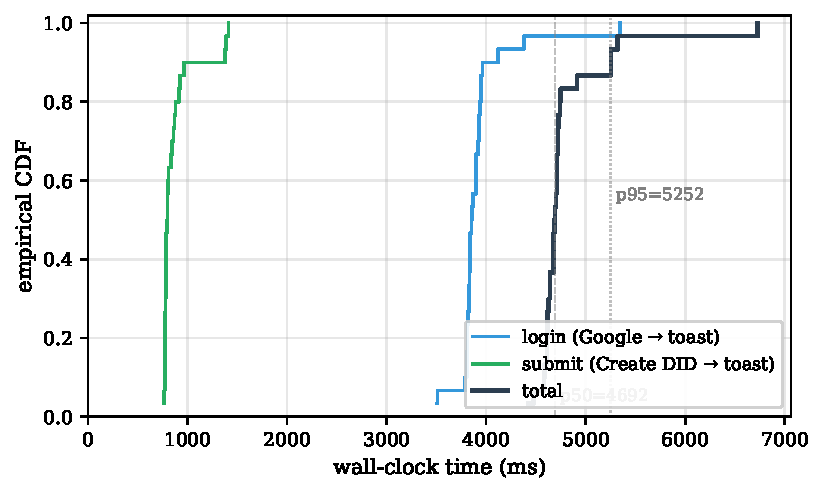
\includegraphics[width=0.85\linewidth]{figures/fig_wall_total_cdf.pdf}
\caption{Empirical CDF of \texttt{wall\_login}, \texttt{wall\_submit},
and \texttt{wall\_total} over $n = 30$ trials under the
persistent-worker backend. Twenty-nine of the thirty trials fall in
$[4{,}428, 5{,}322]$\,ms; the single \texttt{wall\_total} = 6{,}727\,ms
trial is the only outlier and is attributable to one slower Sui DevNet
finality round (its \texttt{wall\_submit} of 1{,}413\,ms versus the
remaining 29-trial median of $796$\,ms), not to the zkLogin pipeline.}
\label{fig:fig_wall_total_cdf}
\end{figure}

% ----------------------------------------------------------------------------
% Distribution Characteristics
% ----------------------------------------------------------------------------
\paragraph{Distribution Characteristics}
\label{sec:e2e-discussion}

Three observations follow immediately from
Table~\ref{tab:e2e-distribution} and Figure~\ref{fig:fig_wall_total_cdf}.

\textbf{(i)~The login phase remains highly reproducible and is unaffected
by the backend optimization.}
\texttt{wall\_login} exhibits CV = 7.9\,\% (sd = 308\,ms around a 3.92\,s
mean), and the mean shifts by only 47\,ms (+1.2\,\%) relative to the
spawn-per-request baseline. This is the expected outcome: the
persistent worker affects only the post-\emph{Create DID} backend code
path, while \texttt{wall\_login} is dominated by an OAuth round-trip,
four real-network salt requests (three of which traverse the
\texttt{us-east-1}\,$\leftrightarrow$\,\texttt{us-west-1} public path),
and an independent ZK-proof generation against the Mysten prover.

\textbf{(ii)~The submit phase is dramatically faster and concentrates
near a single mode.}
\texttt{wall\_submit} drops by 1{,}023\,ms at the mean (\(-54.0\,\%\))
and by 1{,}138\,ms at the median (\(-58.8\,\%\)) compared to the
spawn-per-request baseline. Of the 30 trials, 27 fall below 1{,}000\,ms
(median 796\,ms, sd 184\,ms within this cluster), and only 3 trials
fall in $[1{,}376, 1{,}413]$\,ms. The fast cluster reflects the
post-amortization steady state — the worker's hot caches keep the
in-process backend cost at $\sim$110\,ms — leaving Sui DevNet finality
polling and IPC handling as the only meaningful contributors. The
slow cluster of 3 trials corresponds to occasions where DevNet
finality required two backoff polls rather than one. The contrast
with the spawn-mode bimodal distribution
($\{1{,}380, 1{,}950\}$\,ms clusters caused by Node start-up and SDK
cold-load) demonstrates that process-spawn overhead and SDK
cold-import accounted for the majority of the prior \texttt{wall\_submit}.

\textbf{(iii)~Median total latency is 4.69\,s.}
The p50 of \texttt{wall\_total} is 4{,}688\,ms (down from 5{,}782\,ms
in the spawn baseline, a 1{,}094\,ms reduction). Across the 29
non-outlier trials the empirical maximum is 5{,}322\,ms, corresponding
to p95 (down from 5{,}904\,ms). For 100 sequential DID registrations
under realistic multi-region salt deployment, this corresponds to a
projected end-to-end latency reduction of $\approx 100$\,s
(\(100 \times 1.0\)\,s/DID), establishing the persistent-worker
architecture as a single-largest engineering optimization in the
unmodified-protocol design space.
